\chapter{Monte Carlo Simulation of Thermodynamic Disorder in \CZTS}\label{MC_section}
For this study we have created a custom Monte Carlo code to simulate on-lattice  substitutional disorder amongst copper and zinc ions in {\CZTS} as a function of temperature. In the following sections the methodology applied in the development of the model and methods for quantifying structural disorder will be discussed. Methods for extracting information on band tailing from the disorder will be discussed in section \ref{eris_future_work} as future work.


\section{Mapping the Crystal Structure of { \CZTS } onto a Simple Lattice}\label{mapping}

\begin{figure}[h!]
  \centering
    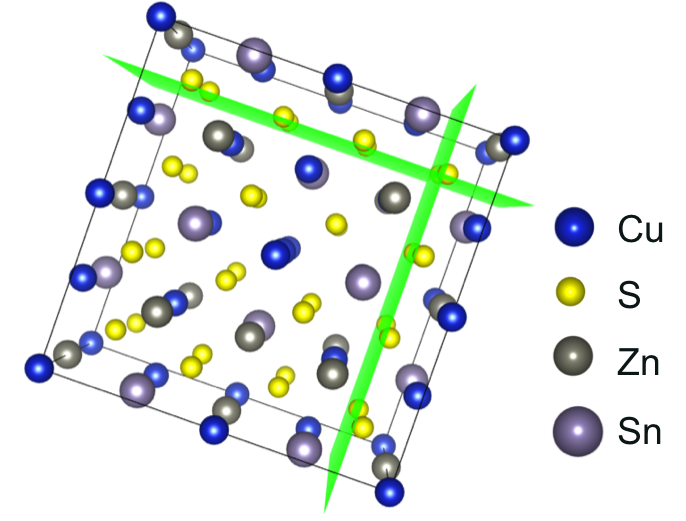
\includegraphics[width=0.5\textwidth]{figures/CZTS_lattice_mapping.png}
    \caption{A supercell of the perfect{ \CZTS } crystal lattice, which can be described by inter-penetrating face-centred cubic sub-lattices: one of metal cations and one of sulfur anions. Green planes are used as guides to the eye to show planes of S anions that form one of the two face-centred cubic sub-lattices.}
  \label{CZTS_lattice_mapping}
\end{figure}

\begin{figure}[h!]
  \centering
    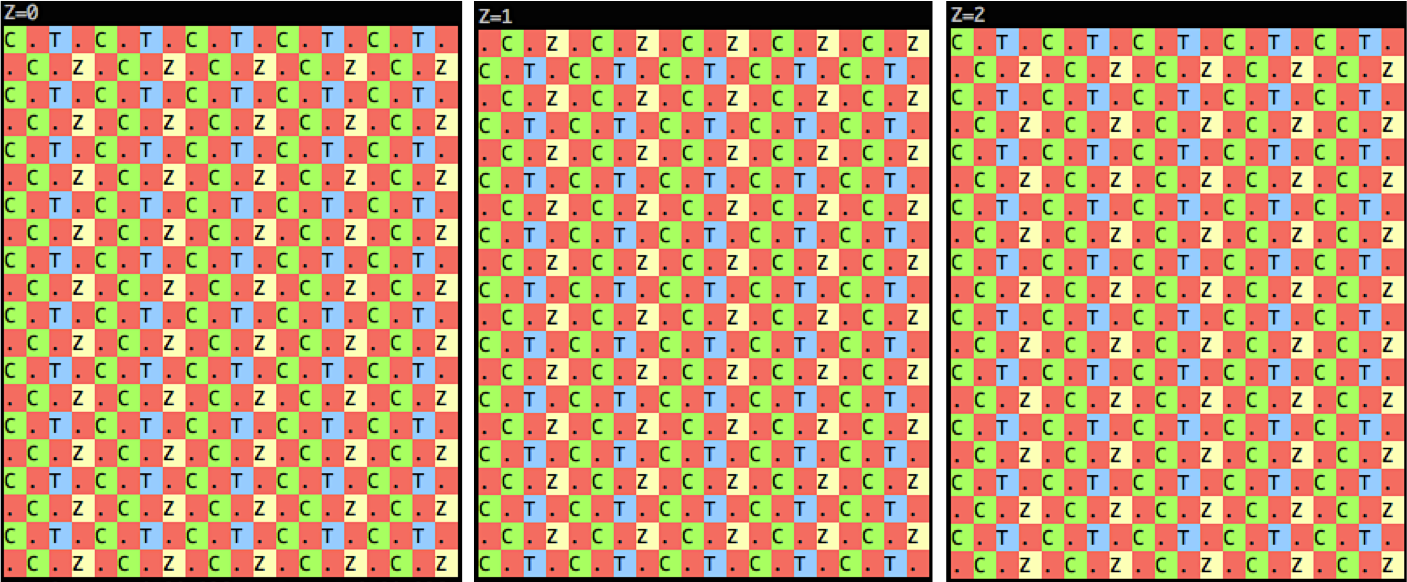
\includegraphics[width=0.95\textwidth]{figures/eris_config_eg.png}
    \caption{A two-dimensional (x-y) slice of a 20x20x20 cation sub-lattice of ordered { \CZTS }. Sulfur anions are neglected from the simulations and the face-centred cubic cation lattice is mapped onto a simple cubic lattice by including empty sites in the lattice. Alternating layers in the z-direction are displaced by one lattice unit in order to reproduce the correct kesterite structure. `C', `Z', `T' and `.' represent copper, zinc, tin and an empty site respectively.}
  \label{eris_config_eg}
\end{figure}

The crystal structure of {\CZTS } can be described by two inter-pentrating face-centred cubic (FCC) lattices: one of metal cations and one of sulfur anions, as shown in figure \ref{CZTS_lattice_mapping}. We consider the sulfur sub-lattice to be stationary because any substitution between ions in the cation sub-lattice and sulfur anion sub-lattice would be energetically infeasible and any substitutions amongst the sulfur anions in that sub-lattice would be energetically equivalent. The sulfur sub-lattice is therefore neglected during the Monte Carlo simulations but incorporated later in calculations of lattice electrostatics. This then reduces the problem of mapping the {\CZTS } crystal structure onto a simple lattice to just one FCC cation lattice. We then map this onto a simple cubic (SC) lattice for our simulations by introducing empty lattice sites into the SC lattice, as shown in figure \ref{eris_config_eg}. Sn ions are also fixed during our simulations to enable us to extract band tailing due to Cu-Zn disorder only. Furthermore, the formation of Sn defects has been predicted to have a considerably higher formation energy than that of $Cu_{Zn}^-$ and $Zn_{Cu}^+$ antisite defects \cite{defect1}.

During our simulation the separation between lattice sites is one lattice unit but this is re-scaled for calculations of lattice electrostatics using our DFT-optimised lattice parameters of $\frac{a}{2}  = \frac{b}{2} = \frac{5.44}{2} \AA$. Where the lattice parameters are divided by 2 as empty sites are placed in between ions to map the FCC structure onto an SC lattice. Figure \ref{CZTS_lattice_scaling} shows flat representations of the crystal structure, with empty lattice sites marked out by crosses. Lattice parameter c for our model will then be approximated to 2a, which is very close to the DFT-optimised value of 10.86 \AA .  

\begin{figure}[h!]
  \centering
    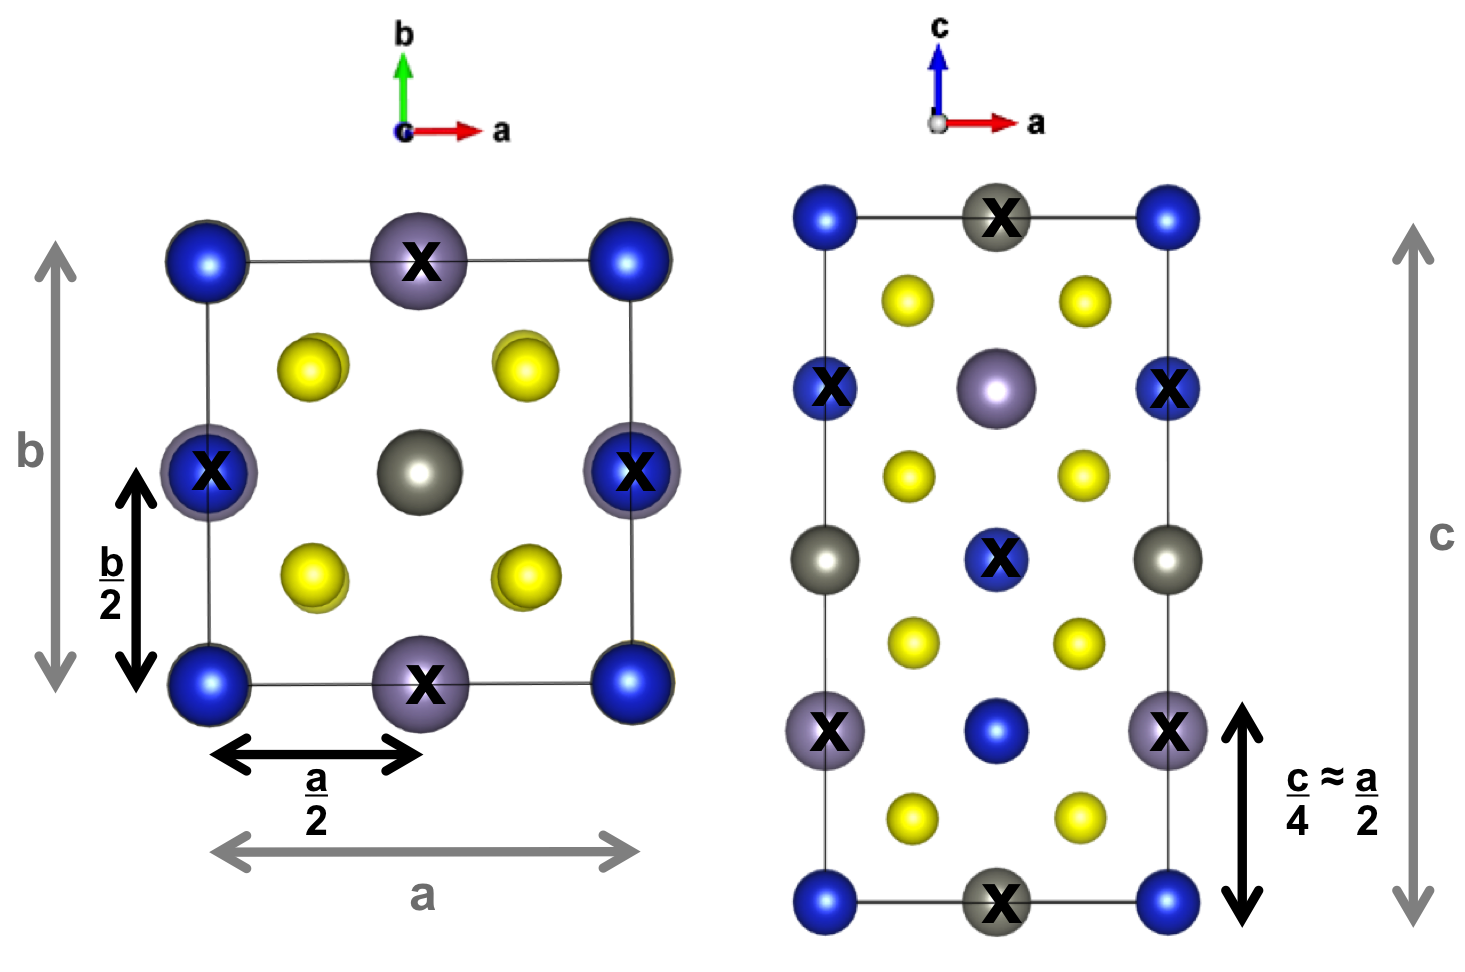
\includegraphics[width=0.9\textwidth]{figures/CZTS_lattice_scaling.png}
    \caption{Visuals of the { \CZTS } crystal structure showing positions of empty sites (denoted by x's) used to map the face-centred cubic lattice of the cations onto a simple cubic lattice. Lattice parameters obtained from hybrid density functional theory geometry optimizations are a = b = 5.43770 {\AA} and c = 10.85670 \AA, and so c is approximately 2a.}
  \label{CZTS_lattice_scaling}
\end{figure}

For some of our simulations, we initialise the system as the cation sub-lattice of the perfectly ordered crystal structure of CZTS. Then for simulations where we want to start from a disordered system, we again take this perfectly ordered initial structure but `shuffle' Cu and Zn ions. An initial configuration of a large SC lattice of perfectly ordered CZTS is generated by producing a supercell of a unit cell of the perfectly ordered structure, where this unit cell was determined by examining the geometry of CZTS one layer at a time in three dimensions. An example of this analysis is shown in figure \ref{unit_cell_eris_supercell}. The smallest unit cell was found to be a 2x2x4 cell when including the gap sites. 

\begin{figure}[h!]
  \centering
    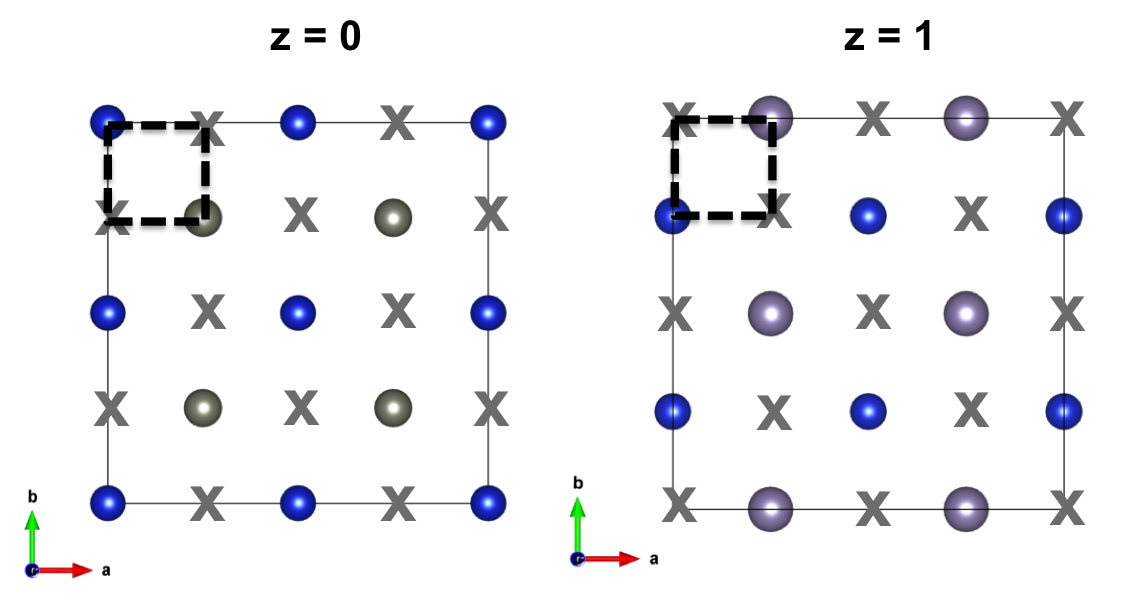
\includegraphics[width=0.9\textwidth]{figures/unit_cell_eris_supercell.png}
    \caption{Some of the single layers of a CZTS supercell used to determine the minimum cation unit cell for constructing supercells in on-lattice Monte Carlo simulations. Here crosses are used to denote the empty sites used in to map a face-centred cubic lattice onto a simple cubic lattice.}
  \label{unit_cell_eris_supercell}
\end{figure}


\section{Monte Carlo Simulation with the Metropolis Algorithm}

The Monte Carlo method can be used to calculate thermodynamic information about a system of N interacting ions represented on a 3D lattice by using classical statistics, considering only two-body forces and assuming that the potential field of an ion is spherically symmetric. If we know the positions of the N interacting ions on the lattice then the potential energy of the system can be calculated using equation \ref{pot_E}, where V is the Coulombic potential between two ions and $d_{ij}$ is the minimum distance between ions i and j \cite{Metropolis}.
\begin{equation}\label{pot_E}
E = \frac{1}{2} \sum_{i=1}^N \sum_{j=1}^N V d_{ij}
\end{equation}
To calculate the properties of the system, the canonical ensemble is used where the temperature, number of ions and volume are all constant. In this ensemble, the equilibrium value for any quantity of interest, B, is given by equation \ref{av}, where $E_\alpha$ is the energy of the system when in state $\alpha$ and $p_\alpha$ is the probability of the system being in state $\alpha$.
\begin{equation}\label{av}
<B> = \frac{ \sum_\alpha e^{-\frac{E_\alpha}{k_bT}} B_\alpha}{ \sum_\alpha e^{-\frac{E_\alpha}{k_bT}}} = \frac{ \sum_\alpha e^{-\frac{E_\alpha}{k_bT}} B_\alpha}{Q} = \sum_\alpha B_\alpha p_\alpha
\end{equation}
\begin{equation}\label{prob}
p_\alpha = \frac{  e^{-\frac{E_\alpha}{k_bT}} }{ \sum_{\alpha} e^{-\frac{E_\alpha}{k_bT}}} =\frac{  e^{-\frac{E_\alpha}{k_bT}} }{Q}
\end{equation}
Q in equation \ref{av} is called the partition function. For most systems calculating the value of the partition function requires the summation over a large number of states. When applying the Monte Carlo method to a system of particles, the summation over discrete states for Q is replaced by a set of integrals. This is shown in equation \ref{MC_av} where $U(\mathbf{r}^N)$ is the potential energy of the system which depends upon the position, \textbf{r}, of the N interacting ions in the system and $Z_{NVT}$ is the configurational integral \cite{Lesar3}.
%\begin{equation}\label{MC_prob}
%p(\mathbf{r}^N) = \frac{  e^{-\frac{U(\mathbf{r}^N)}{k_bT}} }{\int %e^{-\frac{U(\mathbf{r}^N)}{k_bT}} d\mathbf{r}^N}  = \frac{  e^{-\frac{U(\mathbf{r}^N)}%{k_bT}}}{Z_{NVT}} 
%\end{equation}
\begin{equation}\label{MC_av}
<U> = \frac{ \int e^{-\frac{U(\mathbf{r}^N)}{k_bT}} U(\mathbf{r}^N) d\mathbf{r}^N}{\int e^{-\frac{U(\mathbf{r}^N)}{k_bT}} d\mathbf{r}^N}  = \frac{  \int e^{-\frac{U(\mathbf{r}^N)}{k_bT}} U(\mathbf{r}^N) d\mathbf{r}^N}{Z_{NVT}} 
\end{equation}
The configurational integral is over the three coordinates of each ion, as shown in equation \ref{dr}. There are therefore 3N coordinates that define all possible configurations of the system.
\begin{equation}d \mathbf{r}^N = dx_1 dy_1 dz_1 dx_2 dy_2 dz_2... dx_N dy_N dz_N\end{equation}\label{dr}
For a system containing several hundred ions this would be a several-hundred dimensional integral over the configuration space, which would be impractical to carry out by the usual numerical methods. The Monte Carlo method for many-dimensional integrals is used for this purpose \cite{Metropolis}. It is conceptually easiest to think about this method for a one-dimensional integral. This method involves sampling a large number of random points within a region defined by the limits of the integral. The integrated function is then the fraction of points that fall below the curve of the function multiplied by the area of the sampled region. The value obtained becomes a better approximation to the actual value of the integral as the number of random numbers, called Monte Carlo steps (MCS), used to sample the integration region increases. \cite{Lesar3}.

The Standard Monte Carlo method for our system would involve placing each of the N ions at random positions in the lattice to define a random point in the 3N-dimensional configuration space. The energy of the system would then be calculated using equation \ref{pot_E} and the configuration would then be weighted using $e^{-\frac{U(\mathbf{r}^N)}{k_bT}}$ when obtaining the equilibrium value of U. However, many configurations are very improbable so performing this calculation for every possible configuration would be inefficient and unnecessary to sufficiently evaluate the ensemble. The custom Monte Carlo code in this study makes use of the Metropolis modified Monte Carlo scheme \cite{Metropolis}. In this implementation of the Monte Carlo method, instead of choosing configurations randomly and then weighting them, the Metropolis algorithm considers the relative probability of a system being in a new configuration, $\beta$, to that of being in the current configuration, $\alpha$. This is shown in equation \ref{relative_prob}, where $E_\alpha$ is the energy of state $\alpha$ and $E_\beta$ is the energy of state $\beta$.
\begin{equation}\label{relative_prob}
\frac{p_\beta}{p_\alpha} = \frac{  e^{-\frac{E_\alpha}{k_bT}} }{Q} \frac{Q}{  e^{-\frac{E_\alpha}{k_bT}} } = e^{- \frac{E_\beta - E_\alpha}{k_BT}}
\end{equation}
The relative probabilities of the two states are completely determined by the energy 
difference, such that if:
\begin{equation}\label{met}
\Delta E = E_{\beta} - E_{\alpha} \leq 0 \text{   then   } \frac{p_{\beta}}{p_{\alpha}} \geq 1 
\end{equation}
and if
\begin{equation}\label{met2}
\Delta E = E_{\beta} - E_{\alpha} > 0 \text{   then   } \frac{p_{\beta}}{p_{\alpha}} < 1
\end{equation}

The Metropolis algorithm creates a list of configurations through configuration space that has the correct probability distribution. This list is called a trajectory through configuration space. The approach involves making a trial move of the system to a new configuration, in the case of our study this would be a substitution between a Cu and a Zn ion. It is then decided if this new configuration should be added to the trajectory or not based on the probability of the new configuration relative to the current configuration. If the relative probability is  $\geq$ 1, as shown in equation \ref{met}, then the move is accepted and added to the trajectory. However, if the relative probability is $<$ 1 then the move will only be accepted if $e^{-\frac{\Delta E}{k_BT}} \ge$ a random number generated between 0 and 1 \cite{Lesar3}.


\section{Equilibration \& Finite Size Effects}\label{equilibration}
Our Monte Carlo model for Cu-Zn disorder is analogous to the Ising model of a ferromagnet, descriptions of which can be found in many textbooks such as references \citenum{MC} and \citenum{MC_Landau}. In the case of an Ising model, the trial moves in the Metropolis algorithm are spin flips, whereas in our model the trial moves are swaps between Cu and Zn ions. Typically when performing simulations of an Ising model the calculated quantities of interest are the internal energy and average magnetization of the system as a function of temperature obtained by summing over the distribution of atomic spins. In the case of our system, the quantities of interest are the spatial arrangement of the Cu and Zn ions due to thermodynamic substitutions between the two species and the resulting distribution of electrostatic potential across the system for the implications this could have on band tailing. As we fix Sn ions in our simulation we calculate the on-site electrostatic potential for Sn ions to study how the chemical environment of these species is altered by Cu-Zn disorder.
However, before we attempt to extract any information on thermodynamic disorder or the associated band tailing we would predict from such disorder, two important considerations for our model will be firstly to determine if the disordered configuration we obtain is in fact the equilibrated configuration at the given temperature and secondly if finite size effects are having an impact on the system properties we obtain from our simulations.

\begin{figure}[h!]
  \centering
    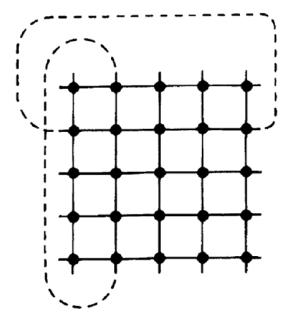
\includegraphics[width=0.4\textwidth]{figures/MC_PBCs.png}
    \caption{Typical periodic boundary conditions for the two-dimensional Ising model. Figure taken from \citenum{MC_Landau}.}
  \label{MC_PBCs}
\end{figure}

As simulations are performed for finite lattices, in order to simulate a bulk system the edges or `boundaries' of the system must be treated carefully. The boundaries can be effectively eliminated through the use of periodic boundary conditions (PBCs). In the case of an Ising model, this means that the first spin in a row interacts with the last spin in the row as if it were a nearest neighbour, and vice versa \cite{MC_Landau}. This principle is illustrated for a two-dimensional system in figure \ref{MC_PBCs}. Although this procedure effectively eliminates boundary effects, the system is still characterized by the finite lattice size, L, which limits the correlation length to $\frac{L}{2}$. Resultant properties of the simulated system may then differ from the bulk system. We therefore will need to perform simulations with increasing system size to look for any differences in the quantities of interest.

\begin{figure}[h!]
  \centering
    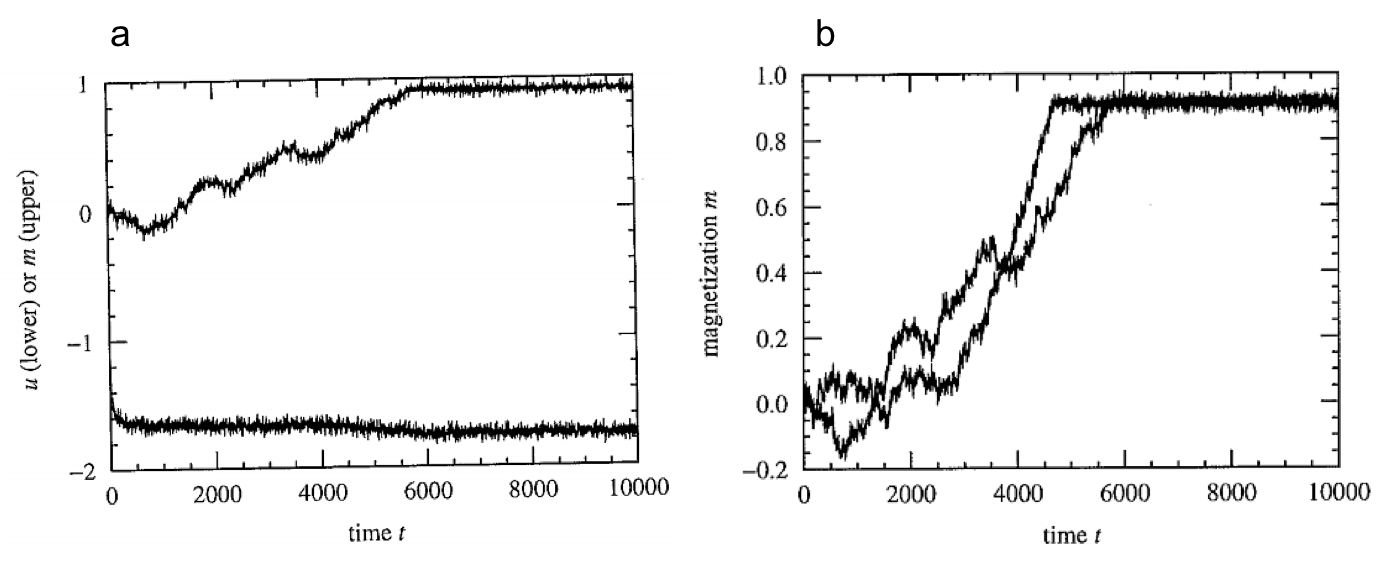
\includegraphics[width=0.9\textwidth]{figures/ising_equil.png}
    \caption{The magnetization (upper curve) and internal energy (lower curve) per site of a two-dimensional Ising model simulated using the Metropolis algorithm (a). Magnetization as a function of time for two different simulations (b). Time is measured in Monte Carlo steps per lattice site. Figures taken from \citenum{MC}.}
  \label{ising_equil}
\end{figure}

Determining if our system has reached equilibration at each temperature however may require a more complicated proceedure. As the Monte Carlo method is stochastic, making use of sampling many times with random numbers in order to determine the minimum energy configuration of the system, the trajectory to reach this final configuration will by nature be random. Therefore, we can draw no conclusions about the properties of our system from evolved states until the final configuration at the particular temperature is reached. Even then we must consider the possibility of our system finding local minima instead of global minima, and therefore giving a false impression of having equilibrated. We therefore are developing methods to check for equilibration before we attempt to extract any thermodynamic properties of our system.

In the case of the Ising model when, for example, determining the average magnetization of a system at a given temperature, the simulation must be run for a suitably long time until the system has come to equilibrium at that temperature. This is referred to as the equilibration time and the point at which a system has attained equilibrium can be defined as being when the average probability of finding the system in any particular state $\alpha$ is proportional to the Boltzmann weight of that state, $e^{-\frac{E_\alpha}{k_bT}}$. Once the system has equilibrated, the quantity of interest such as the magnetization must then be measured again over a suitably long time and averaged \cite{MC}. 
To gauge if a system has reached equilibrium, in the case of the Ising model, it is common practice to run the simulation for a large number of Monte Carlo steps (MCS) (where one MCS corresponds to attempting a trial spin-flip at all sites in the system once) and looking for how the value of a quantity of interest, such as the average magnetization across the system, changes with increasing number of MCS as the simulation progresses. Equilibration is often considered as the point at which the value of a quantity of interest, which initially changes by a large amount, eventually converges to fluctuating about a steady average value. An example of this is shown in figure \ref{ising_equil}a. This is dependent upon the principle that a system in equilibrium spends the overwhelming majority of its time in a small subset of states in which its properties take a narrow range of values \cite{MC}. Provided the simulation is allowed to run for a sufficiently long time to reach this global minimum energy (or equilibrium) configuration and that the system does not become stuck in a local minimum state, the final configuration for a given system at a given temperature should always be the same regardless of the initial configuration of the simulation, this point is illustrated in figure \ref{ising_equil}b.

\begin{figure}[h!]
  \centering
    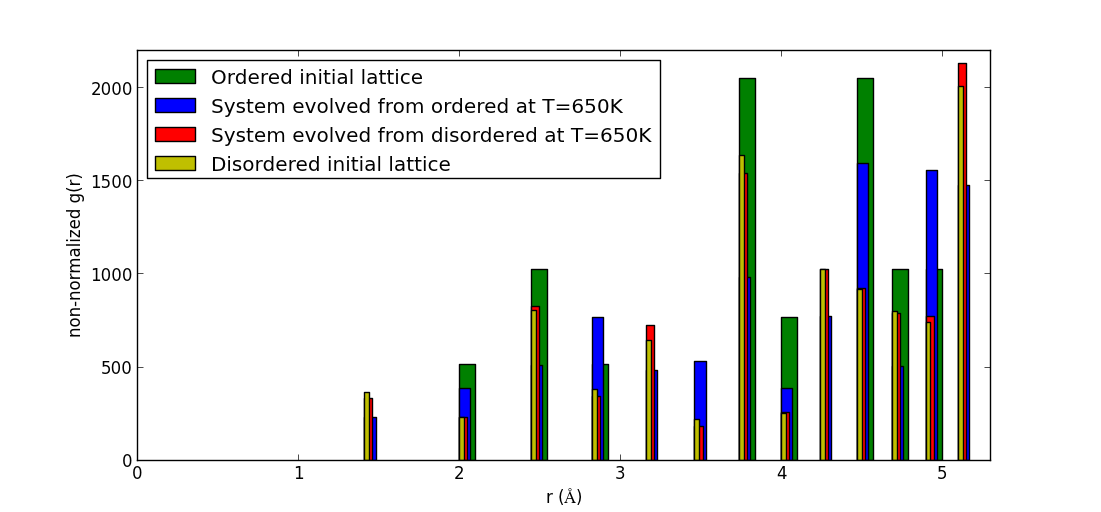
\includegraphics[width=1.0\textwidth]{figures/RDF_Z-Z_equil_check.png}
    \caption{The radial distribution function (RDF) between pairs of zinc ions in {\CZTS} before normalization. RDFs of an initial perfectly ordered lattice are plotted with that of a disordered initial lattice as reference points as well as systems that have been evolved from both of these initial configurations at T=650K. Widths of the bars plotted are arbitrarily chosen to ensure all data is visible.}
  \label{RDF_Z-Z_equil_check}
\end{figure}

Using this principle, one way to determine if our system has reached its equilibrium configuration could be to use the perfectly ordered or disordered initial lattice configurations that were discussed at the end of section \ref{mapping}. Both of these initial configurations, if the simulation is allowed to evolve over a suitable number of MCS, should eventually result in the same equilibrium system configuration. It would be difficult to distinguish differences in the atomic arrangement of one 3D lattice to another by eye, therefore comparisons of the radial distribution function (RDF) for each configuration as it evolves from either an ordered or disordered initial configuration will be made. Using RDFs for structural analysis will be discussed further in section \ref{RDF_methods}, but for the present discussion, the point after which the RDF of the system evolved from an ordered initial lattice converges to being the same as that of a system evolved from a disordered initial lattice could be one way to determine if the system has reached its equilibrium configuration. 

An example of this analysis is shown in figure \ref{RDF_Z-Z_equil_check}. So far, we have seen that the system evolves much faster (in terms of number of MCS as opposed to time) when starting from an initially ordered configuration than an initially disordered configuration. This could be explained by it being more entropically favourable for a system to move away from a highly ordered system than to move from a disordered configuration to a more ordered configuration. 
%As the difference in the RDF peaks can be difficult to gauge by eye and as our system is on lattice, we are also summing over the square of the difference in the RDF peak intensities at each value of r to quantify the difference in the distributions. 
So far in our study we have found that the system evolution from a disordered initial configuration is possibly too slow for comparisons between this simulation and that from an ordered initial configuration to be a feasible method to check for equilibration.

\begin{figure}[h!]
  \centering
    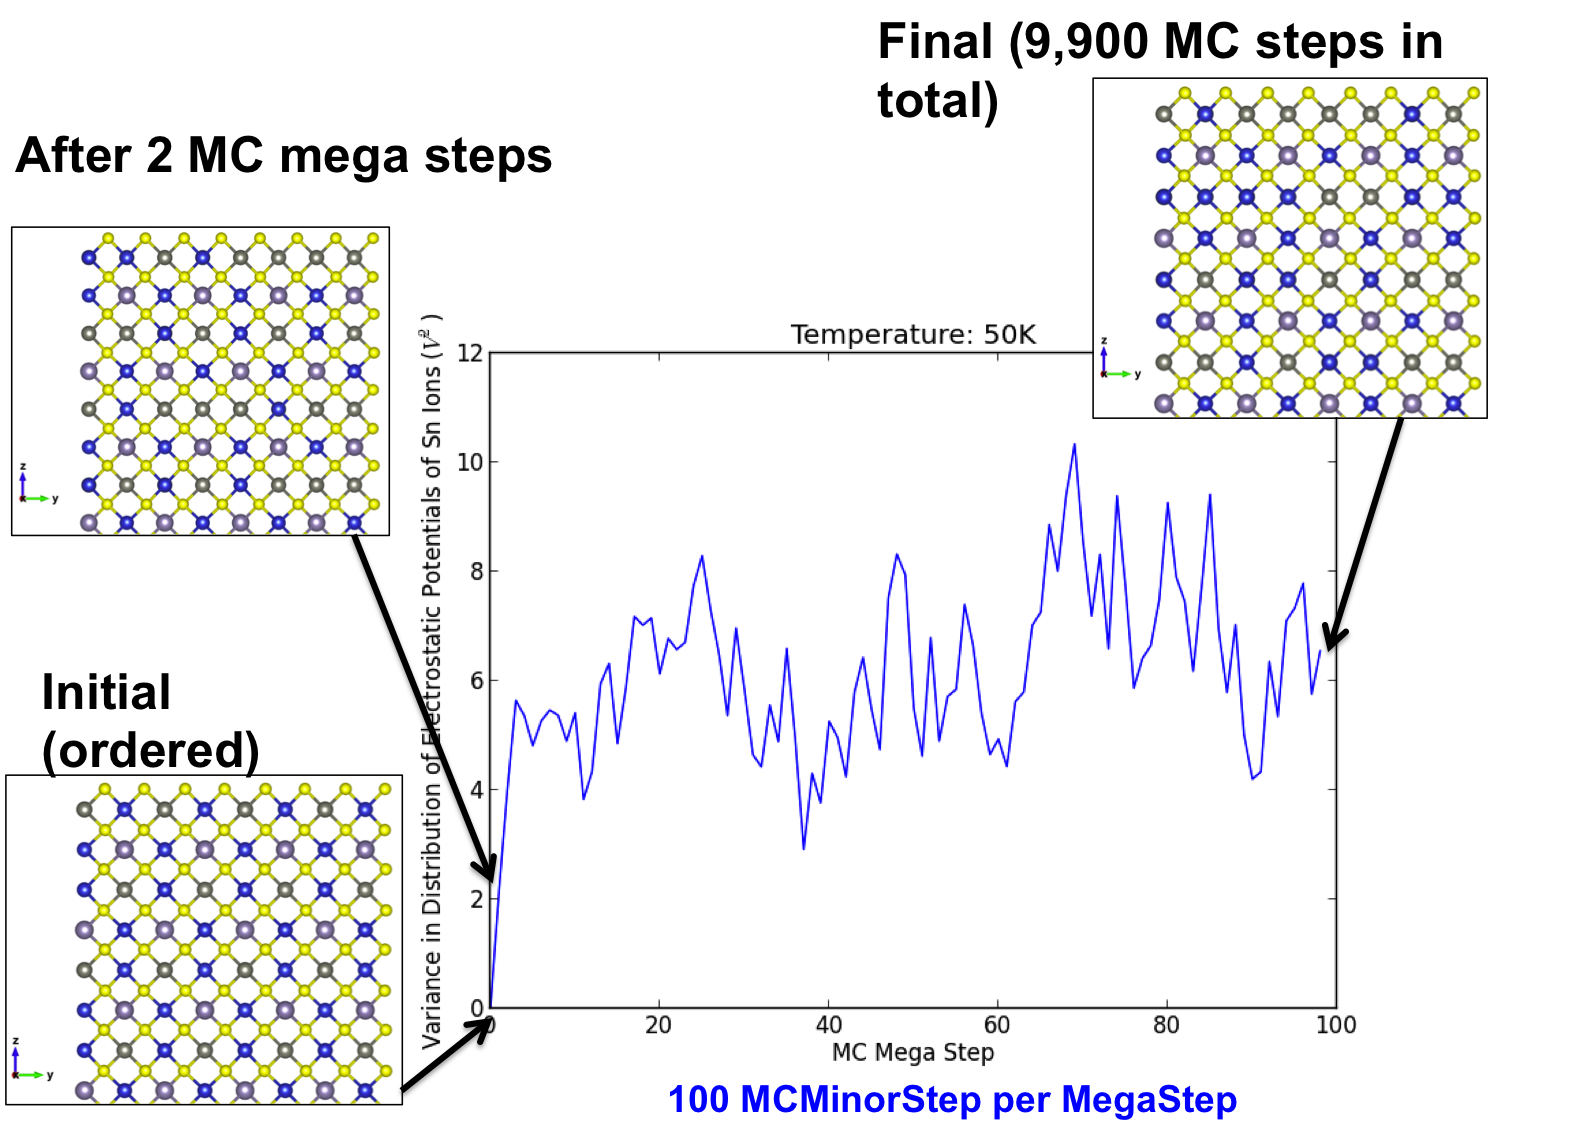
\includegraphics[width=1.0\textwidth]{figures/50K_100Minor-per-mega+visuals.png}
    \caption{Variance in the distribution of Sn ions in a system of containing 128 Sn ions, where the system is evolved from an initially perfectly ordered lattice. Each `MC Mega Step' corresponds to 100 Monte Carlo steps, which for our simulations are substitutions between Cu and Zn ions. Representative two-dimensional slices of the system are shown during system evolution from the perfectly ordered lattice, which when viewed along this crystallographic direction is alternating layers of Cu-Zn and Cu-Sn ions.}
  \label{variance_with_MCS}
\end{figure}

Another method to check for equilibration is analogous to that shown in figure \ref{ising_equil}a for the Ising model. In the case of our system, it is the distribution of the electrostatic potential at Sn sites in the system that is of interest so one possible method to check for equilibration could be to look for a point after which the variance of the distribution of electrostatic potentials across the system has reached a steady value. An example of this analysis is shown in figure \ref{variance_with_MCS}, where the system was evolved from an ordered initial configuration. In contrast to the disordered initial configuration, systems evolved from an initially perfectly ordered lattice appear to equilibrate quickly where in figure \ref{variance_with_MCS}, each `MC Mega Step' corresponds to 100 Monte Carlo steps (MCS). The figure shows the variance evolving from the initially perfectly ordered system, in which there is only one distinct crystallographic environment for Sn and so the variance is zero, to fluctuating around a finite value. Figure \ref{variance_with_MCS_1000} shows the same simulation performed with 1000 MCS per data point.

\begin{figure}[h!]
  \centering
    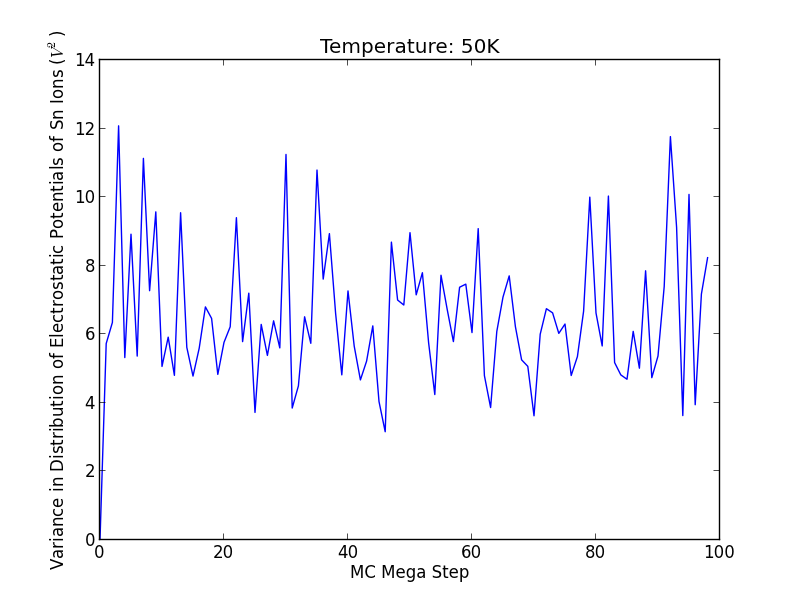
\includegraphics[width=0.75\textwidth]{figures/1000Minor_per_Mega2.png}
    \caption{Variance in the distribution of Sn ions in a system of containing 128 Sn ions, where the system is evolved from an initially perfectly ordered lattice. Each 'MC Mega Step' corresponds to 1000 Monte Carlo steps, which for our simulations are substitutions between Cu and Zn ions.}
  \label{variance_with_MCS_1000}
\end{figure}


\section{Multi-Scale Approach with Density Functional Theory}\label{MC_DFT}
Equation \ref{eris_interaction} can be used to calculate the electrostatic interaction between a pairs of ions, where $q_1$ and $q_2$ are the bare formal charges, r is the separation of the point charges and $\epsilon_r$ is the bulk static relative dielectric constant. The interaction between all pairs of ions within the system are summed over when calculating the change in the energy of the system after performing a trial move in our Monte Carlo simulations.
\begin{equation}\label{eris_interaction}
E_{electrostatic} = \frac{q_1q_2}{4\pi\epsilon_0\epsilon_r}e^2\frac{1}{r} = q_1q_2 I_{electrostatic}
\end{equation}
We separate out the parameter $I_{electrostatic}$ in our simulations. The value is first calculated considering a purely classical, electrostatic case where only the bare formal charges on the ions are considered and the bulk dielectric constant of { \CZTS } is used. Using a value of 13.2 for $\epsilon_r$ and 3.8 $\AA$ for r, which is the separation of nearest-neighbour Cu-Zn ions, gives a value of -0.284 eV for $I_{electrostatic}$.
This treatment however only accounts for the Coulombic interaction between the point charges and neglects any changes in the electronic structure during defect formation. The screening effect of the electronic structure would be more significant for the microscopic dielectric constant than for the bulk, macroscopic dielectric constant.
In this study therefore we scale the interaction energy, $I_{interaction}$, in the simulations by comparing the formation energy of a nearest-neighbour Cu-Zn anti-site defect pair calculated using the classical code GULP to that obtained using quantum mechanical hybrid-density functional theory and the VASP code, where effects of the electronic structure are included in the calculation. This calculation was performed in a previous study, but details of the calculation are included in Appendix \ref{Cu-Zn_defects_calc}. We found that the defect formation energy obtained using VASP was approximately 1.5 times that obtained with GULP, we therefore scaled the interaction energy by the same amount and so $I_{DFT} = 1.5 \times I_{electrostatic} = - 0.425$ eV. Through doing this we aim to scale the macroscopic dielectric constant to be closer to the value of the microscopic dielectric constant.

\section{Spatial Extent of Disorder Amongst Cu \& Zn Ions}
Monte Carlo simulations of thermodynamic substitutions between Cu and Zn ions  will be allowed to evolve until the equilibrium configuration in terms of the arrangement of Cu and Zn atoms at the given temperature is reached, which was discussed in section \ref{equilibration}. The electrostatic potential at each site in the lattice will then be calculated for later analysis of the distribution of electrostatic potential of Sn ions across the system when extracting information on band tailing due to Cu-Zn disorder. The methodology for this will be discussed as future work in section \ref{eris_future-work}. Figure \ref{eris_spatial_disorder} shows an example of outputs from our simulations, where the T = 0K spatial arrangement of cations in figure \ref{eris_spatial_disorder}a corresponds to the perfectly ordered system and the T= 200K configuration in figure \ref{eris_spatial_disorder}b shows spatial clustering of Cu and Zn ions as the system has been allowed to evolve at a finite temperature.

\begin{figure}[h!]
  \centering
    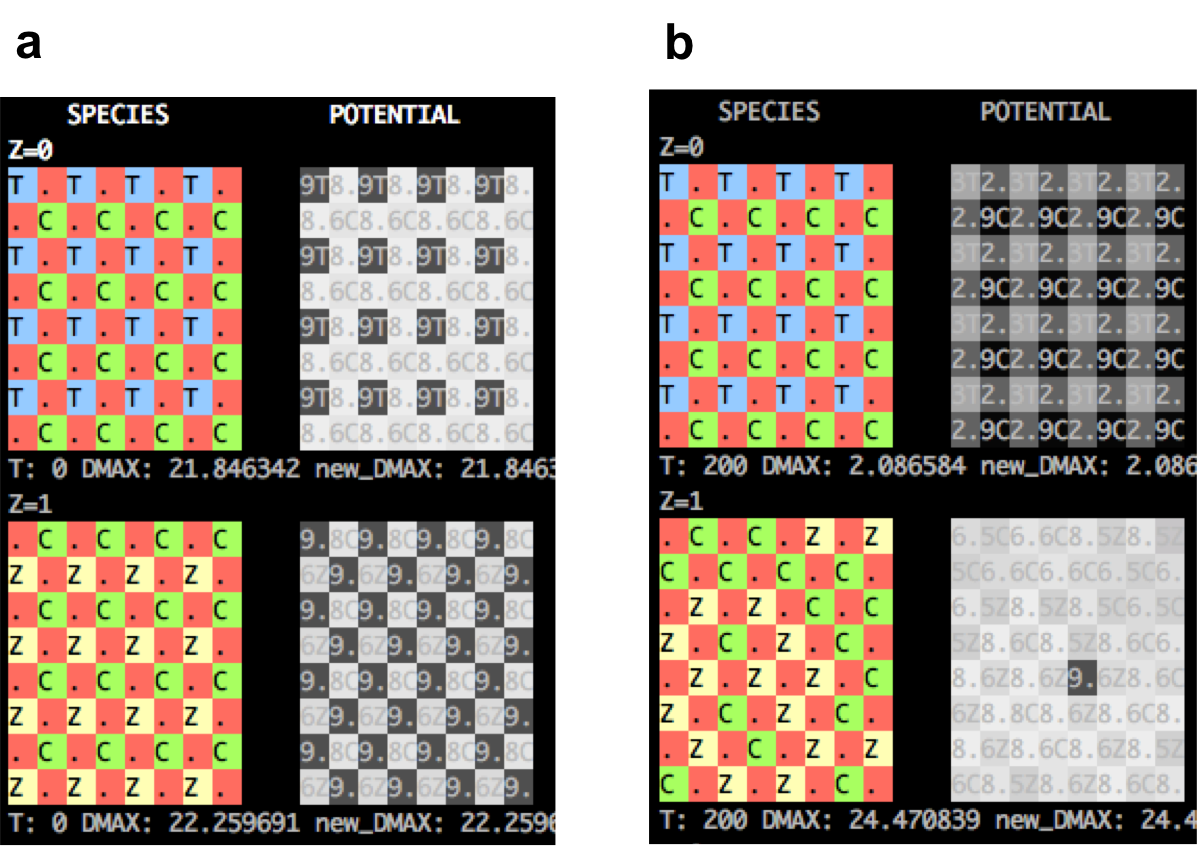
\includegraphics[width=0.9\textwidth]{figures/eris_spatial_disorder.png}
    \caption{Example outputs from Eris Monte Carlo simulations of Cu-Zn disorder from an initially ordered lattice showing the top two layers of the lattice when simulations are performed at temperatures T = 0K (a) and at T = 200K (b).}
  \label{eris_spatial_disorder}
\end{figure}

\section{Quantification of Disorder Using Radial Distribution Functions}\label{RDF_methods}
%\begin{itemize}
%\item Brief overview of what an RDF is
%\item See new lab book and make figures to explain
%\item Reproducing GS: Cu-Zn RDF first peak to describe Cu Zn Cu layer, Cu-Sn RDF first peak to describe Cu Sn Cu layer nearest neighbours
%\item Using RDFs from initial, perfectly ordered system as a reference point: Cu-Sn and Cu-Zn perfectly overlayed, but expect to separate with disorder. First peak (near-neighbours) for Cu-Sn should remain same as Sn is fixed, but Cu-Zn first peak will change as will subsequent peaks for both.
%\item Need to normalize to recover coordination number for first peak?
%\item Increasing intensity of new nearest neighbour Cu-Cu and Zn-Zn peaks for disordered systems with increasing disorder
%\end{itemize}

\begin{figure}[h!]
  \centering
    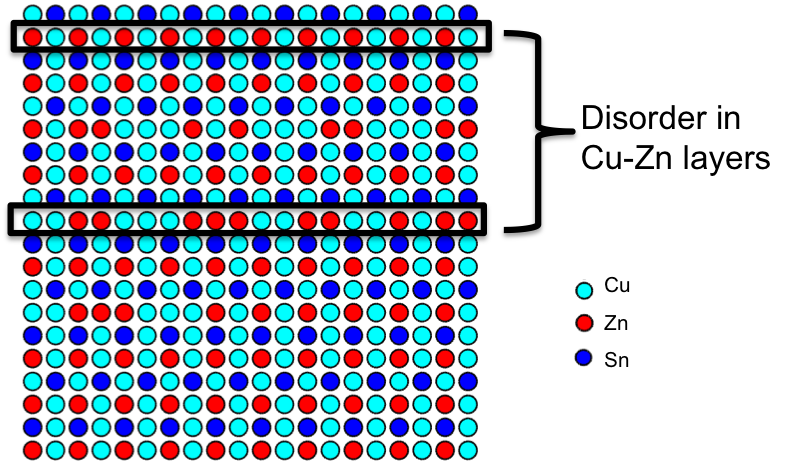
\includegraphics[width=0.8\textwidth]{figures/Cu-Zn_disorder.png}
    \caption{A 2D slice of a disordered configuration of the cation sub-lattice of {\CZTS}, where the top highlighted layer shows an example of perfectly ordered alternating Cu-Zn pattern and the second layer shows an example of a disordered layer.}
  \label{Cu-Zn_disorder}
\end{figure}

In order to analyse the extent of disorder in resulting configurations from our simulations, we plan to use radial distribution functions (RDFs). The RDF of a system of particles describes how density varies as a function of distance from a reference particle. In our study we will use the RDF of particular pairs of species to study how the arrangement of Cu and Zn ions varies across the whole system as a result of thermodynamic disorder.
%The crystal structure of {\CZTS } can be described by alternating layers of Cu-Zn and Cu-Sn \cite{Schorr}, as shown in figure \ref{CZTS_cell}. For the unit cells generated by eris, this corresponds to when the system is viewed along the x-axis and as we fix Sn ions in our simulations, we would expect this direction to always have this same repeating pattern when the system is perfectly ordered. The ordering of ions along this direction therefore could be used as one of our order parameters. However, we should first check that our system crystallises in the same direction as we would expect it to by performing simulations from an initial randomized configuration until the ground state crystal structure is recovered at low temperatures. This may require a simulated annealing approach where a system is equilibrated at a higher temperature and this final equilibrated configuration is then used as the initial configuration for a subsequent simulation performed at a lower temperature until an equilibrated configuration at the desired low temperature is obtained.
The simplest way to quantify disorder could be to use the nearest-neighbour RDF peak of the Cu-Cu or Zn-Zn RDFs as an increase in disorder is associated with clustering of two or more Cu or Zn species together, as shown in figure \ref{Cu-Zn_disorder}. Therefore, when comparing to the RDF of a perfectly ordered system, we could expect a new nearest-neighbour peak to emerge in the Cu-Cu and Zn-Zn RDFs, which will increase in intensity as the regions of clusters of Cu and Zn increase in cluster-size and occur more frequently with disorder. This can be seen in figure \ref{RDF_Z-Z} of the Zn-Zn RDF where a new nearest neighbour peak emerges in the disordered configurations, which was not present for the ordered initial configuration, and the peak appears to increase in intensity going from a system that has been evolved from an initially ordered configuration compared to the disordered initial configuration. This analysis will not entirely capture the disorder process but could be used to quantify the initial disordering from a perfectly ordered system. Ideas for other methods to quantify disorder will be discussed as future work in section \ref{eris_future_work}.

\begin{figure}[h!]
  \centering
    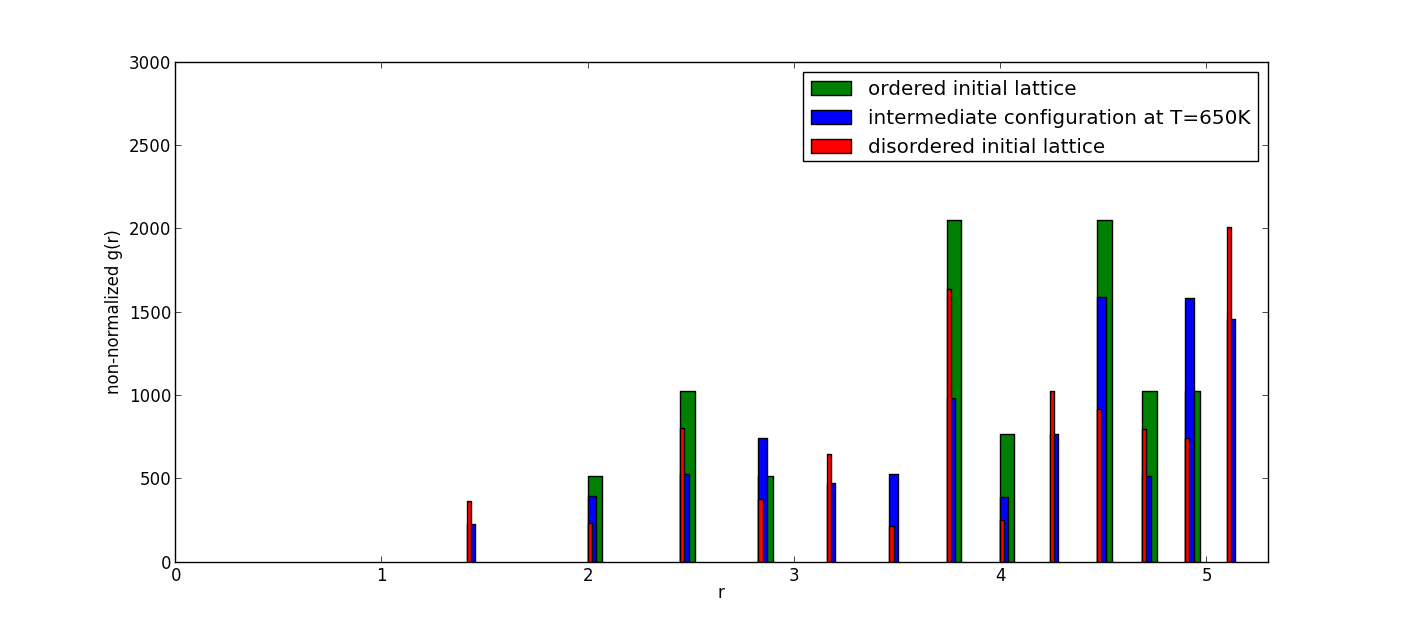
\includegraphics[width=1.0\textwidth]{figures/RDF_Z-Z.png}
    \caption{The radial distribution function (RDF) between pairs of zinc ions in {\CZTS} before normalization. RDFs of an initial perfectly ordered lattice are plotted with that of a disordered initial lattice as well as a system that started from an initially ordered lattice and has been allowed to evolve at T=650K but note that the system may not yet have reached the equilibrium configuration for the given temperature. Widths of the bars plotted are arbitrarily chosen to ensure all data is visible.}
  \label{RDF_Z-Z}
\end{figure}



%\section{Band Tailing from the Distribution of Electrostatic Potential}\label{band_tail_methods}
%Discuss using Sn distribution and extract tails? Show e.g. R plot? See lab book notes + see what Aron and Jarv say

%\begin{figure}[h!]
%  \centering
 %   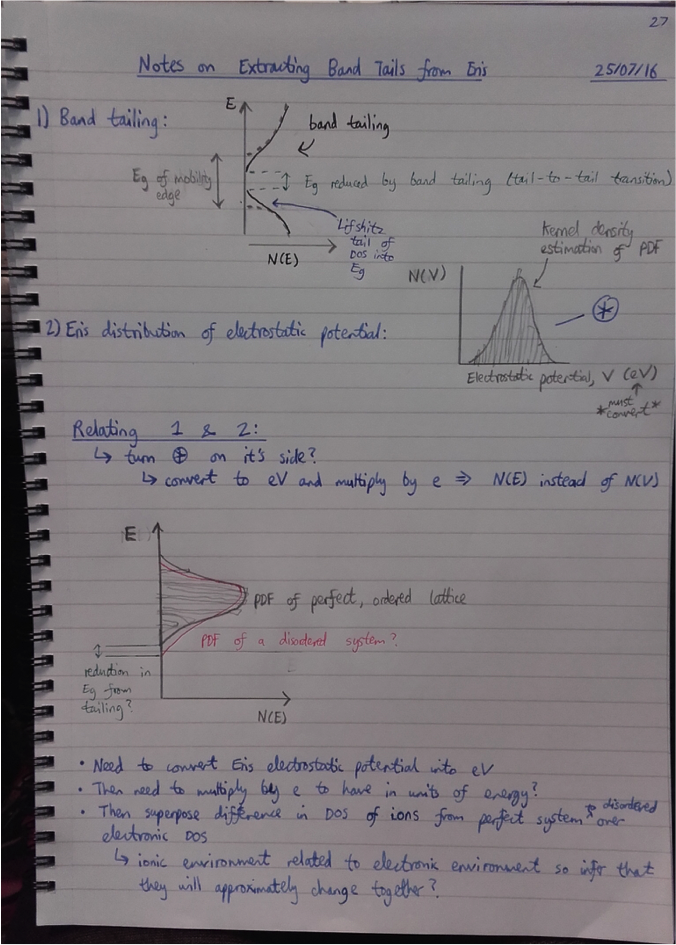
\includegraphics[width=1.0\textwidth]{figures/band_tails_notes.png}
  %  \caption{Placeholder for actual notes! (Wait for feedback)}
 % \label{band_tail_notes}
%\end{figure}


